\section{Related Work}
\label{sec:related_works}
\vspace{-1mm}


\begin{figure*}[t]
\centering
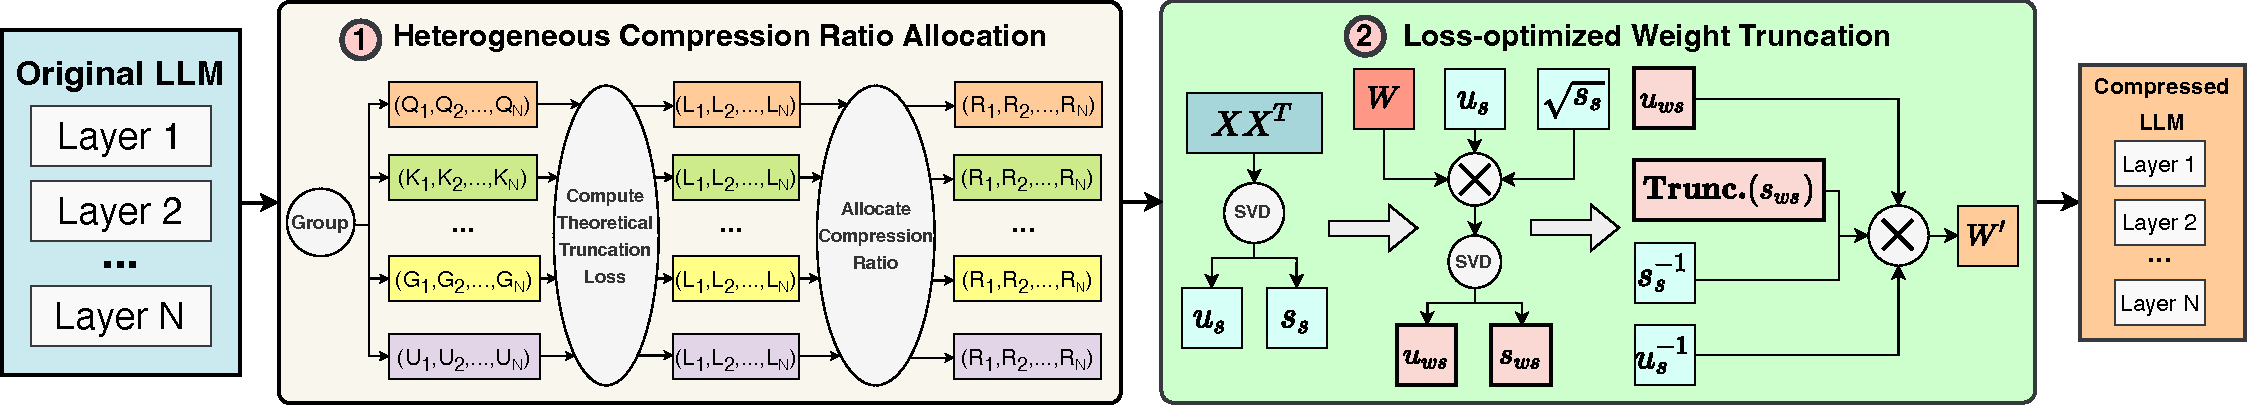
\includegraphics[width=1\textwidth]{Figures/Framework.pdf}
\caption{Overview of \sysname.}
\label{fig:framework}
\end{figure*}


\subsection{Large Language Model Compression}
\label{subsc:large_language_model_compression}
Large Language Models (LLMs) typically contain billions of parameters, making traditional model compression techniques impractical due to the need for resource-intensive retraining. To address this, post-training methods that bypass retraining during compression have been developed. These methods generally fall into four categories: unstructured pruning, structured pruning, quantization, and low-rank approximation. 
%
Unstructured pruning~\citep{DBLP:conf/icml/FrantarA23} sets the individual weight values to zero without changing the overall architecture. However, its irregular sparsity is feasible only for speedups or memory savings on certain hardware. 
%
In contrast, structured pruning~\citep{DBLP:conf/nips/MaFW23,DBLP:conf/iclr/AshkboosCNHH24,DBLP:journals/corr/abs-2406-10594} removes entire channels from LLMs, simplifying hardware implementation but often suffering from accuracy degradation. 
%
Quantization~\citep{DBLP:journals/corr/abs-2210-17323,DBLP:journals/corr/abs-2411-07762} reduces the precision of the weight matrices for compression. However, it often fails to provide the desired inference speedups~\citep{DBLP:journals/corr/abs-2405-04532} and offers a limited range of compression options—typically between 2 to 8 bits—which hinders optimal memory utilization. Recent efforts~\citep{DBLP:conf/iclr/YuanSD24, DBLP:conf/icml/HuangLQLZ0M024} have explored 1-bit post-training quantization. Nevertheless, these approaches still suffer from accuracy drop, indicating that 1-bit quantization is still challenging in LLM compression.

\subsection{SVD for LLM Compression}
Singular Value Decomposition (SVD) reduces matrix sizes by truncating the smallest singular values. It then constructs two smaller, lower-rank matrices to approximate the original matrix~\citep{GOLUB1987317}. SVD is also feasible for LLM~\citep{DBLP:conf/iclr/HsuHCLSJ22, DBLP:journals/corr/abs-2312-05821, DBLP:journals/corr/abs-2403-07378,DBLP:journals/corr/abs-2408-09632}. To ensure better compression performance, existing post-training SVD-based LLM compression methods attempt to lower the truncation loss $L$ in the form of Frobenius norm as follows during LLM compression:

\begin{equation}
    L = ||WX-W'X||_F 
    \label{eq:t1}
\end{equation}

\noindent where $W$ is the weight matrix of the original LLM, $X$ is the activation of $W$, and $W'$ is the compressed low-ranking weight matrix. 
% %
% and many SVD-based compression techniques have been proposed. 
For example,
%\citet{DBLP:conf/iclr/HsuHCLSJ22} propose FWSVD which introduces Fisher information to weigh the importance of parameters.
%
\citet{DBLP:journals/corr/abs-2312-05821} propose ASVD, which scales the weight matrix using a diagonal matrix to normalize the impact of input channels on the weights to reduce the truncation loss. 
%
\citet{DBLP:journals/corr/abs-2403-07378} make further advancement by whitening the input matrix to mitigate its impact on SVD truncation with the guarantee of minimal theoretical truncation loss. 
%
Despite these progresses, existing methods still suffer from high truncation loss in practice, leading to accuracy degradation.
%, which severely hinders their real-world application.